\documentclass{edm_template}
%\documentclass[11pt,twocolumn]{article}
\usepackage{amsmath}
\usepackage{graphicx}
%\usepackage{xcolor}
%\usepackage{svg}
\usepackage{tikz}
\usepackage{algorithmic}
%\usepackage{adjustbox}
\usepackage{paralist}
\usepackage{array}
\usepackage{apacite}
\usepackage{multirow}
\usepackage{dcolumn}
\usepackage{array}
\usepackage{kbordermatrix}
\usepackage{balance}
\usepackage{float}
\DeclareMathOperator*{\argmax}{arg\,max}
    
\begin{document}

\title{An Empirical Research on Identifiability and Q-matrix Design for DINA model}
\numberofauthors{2}
\author{
\alignauthor
Peng Xu\\
       \affaddr{Polytechnique Montreal}\\
       \email{\large\sffamily peng.xu@polymtl.ca}
\alignauthor
Michel C. Desmarais\\
       \affaddr{Polytechnique Montreal}\\
       \email{\large\sffamily michel.desmarais@polymtl.ca}
}
\maketitle

\begin{abstract}
In most contexts of student skills assessment, whether the test material is administered by the teacher or within a learning environment, there is a strong incentive to minimize the number of questions or exercises administered in order to get an accurate assessment.  This minimization objective can be framed as a Q-matrix design problem: given a set of skills to assess and a fixed number of question items, determine the optimal set of items, out of a potentially large pool, that will yield the most accurate assessment.  In recent years, the Q-matrix identifiability under DINA/DINO models has been proposed as a guiding principle for that purpose.  We empirically investigate the extent to which identifiability can serve that purpose. Identifiability of Q-matrices is studied throughout a range of conditions in an effort to measure and understand its relation to student skills assessment.  We compare identifiability to other Q-matrix design principles through simulation studies of skills assessment with both synthetic and real data.
\end{abstract}
%%%%%%%%%%%%%%%%%%%%%%%%%%%%%%%%%%%%%%%%%%%%%%%%%%%%%%%%%%%%%%%%%%%%%%%%%%%%%
\section{Introduction}
Q-matrix based models are widely researched during recent years in educational data mining. Among all of them, DINA model is the most used and discussed. Most of these research are focused on one of the 2 following problems. The first one is the Q-matrix validation problem, that is, to improve or validate an expert-given Q-matrix \cite{de2015general, chiu2013statistical, desmarais2013matrix}. The other one is the Q-matrix derivation problem, that is, to directly derive a Q-matrix out of the test result matrix \cite{barnes2010novel, liu2012data, desmarais2015combining, xu2016boosted}. During the investigation of these two problems, a fundamental question has been proposed, the identifiability of model parameters, especially the Q-matrix. Detailed statistical analysis has been made under the DINA/DINO situation, which was first discussed under the situation that slip and guess is zero\cite{chiu2009cluster}, and then the case that slip and guess exist but is known\cite{liu2013theory}, and finally the case that slip and guess is unknown\cite{chen2015statistical}. 

However, how do we use the conditions offered by the discussion to guide our educational test? First, the discussion is centered around the identifiability on Q-matrix, not on the identifiability of students, which is also a critical problem \cite{beck2007identifiability}. Fortunately, for the case slip and guess are known, the identifiability of the parameters $p$ are also given\cite{chen2015statistical}.  
\section{Identifiability}

The general idea behind identifiability is that two or more configurations of model parameters can be considered as equivalent.  Sets of parameters will be considered equivalent if, for example, their likelihood are equal given a data set.  Or, conversely, if they are susceptible to generate data having the same characteristics of interest (see~\citeNP{doroudi2017misidentified}, for more details).

The issue of identifiability for student skills assessment was first raised for the Bayesian Knowledge Tracing (BKT) model by \citeNP{beck2007identifiability} and later discussed by \citeNP{doroudi2017misidentified}, and \citeNP{van2013properties}.  In this paper, we consider the identifiability of the Q-matrix which was studied by \citeNP{xu2015identifiability} \citeNP{qin2015model}.  

Identifiability of model parameters is a general concept for statistical models, its general definition is,

\textbf{Definition} \cite{casella2002statistical} A parameter $\theta$ for a family of distribution ${f(x|\theta: \theta \in \Theta}$ is identifiable if distinct values of $\theta$ correspond to distinct pdfs or pmfs. That is, if $\theta \neq \theta^{\prime}$, then $f(x|\theta)$ is not the same function of $x$ as $f(x|\theta^{\prime})$.

However, for Q-matrix related model, since exchanging columns does not yield an essentially different Q-matrix. During the research of \citeA{xu2015identifiability}, the identifiability of Q-matrix has been redefined.

\textbf{Definition} \cite{xu2015identifiability} We write $Q \sim Q^{\prime}$ if and only if $Q$ and $Q^{\prime}$ have identical column vectors that can be arranged in different orders. We say that $Q$ is identifiable if there exists an estimator $\hat{Q}$ such that $\lim_{N\to\infty} P(\hat{Q} \sim Q) = 1$.

\textbf{Definition} \cite{xu2015identifiability}  The matrix $Q$ is complete meaning that ${{e_{i}:i=1,...k}} \subset R_{Q}$, where $R_{Q}$ is the set of row vectors of $Q$ and $e_{i}$ is a row vector such that the $i$-th element is one and the rest are zero.

\textbf{Proposition} \cite{xu2015identifiability} Under the DINA and DINO models, with $Q$, $s$ and $g$ being known, the population proportional parameter $p$ is identifiable if and only if $Q$ is complete.

\section{Experiment}
All experiments consider the situation that slip and guess are already known.

\subsection{Experiment 1: Comparison of three strategies}
In this experiment, we compare three different Q-matrix design strategies. They are all based on repetition of a pool of q-vectors.

Strategy 1: Using the identifiability condition. Only repeated using the vectors ${e_{i}:i=1,...k}$.Q-matrix used in this strategy is denoted as Q-matrix 1.

Strategy 2: Using the vectors ${e_{i}:i=1,...k}$ plus a all-one vector $(1,1,1)$ or $(1,1,1,1)$. In this way it forms an orthogonal array, which is a commonly seen design of experiments. Q-matrix used in this strategy is denoted as Q-matrix 2.

Strategy 3: Repeated using all q-vectors.Q-matrix used in this strategy is denoted as Q-matrix 3.

For the three skill case, all these three Q-matrices have been shown below. 

\parbox{.5\columnwidth}{
\hfil Q-matrix 1 \hfil\\
\kbordermatrix{
	& k_1 &k_2 & k_3\\
q_1 & 1 & 0 & 0 \\
q_2 & 0 & 1 & 0 \\
q_3 & 0 & 0 & 1 \\
... & ... & ... & ... &\\
q_{19} & 1 & 0 & 0 \\
q_{20} & 0 & 1 & 0 \\
q_{21} & 0 & 0 & 1 \\
}}
\parbox{.5\columnwidth}{
\hfil Q-matrix 2 \hfil\\
\kbordermatrix{
	& k_1 &k_2 & k_3\\
q_1 & 1 & 0 & 0 \\
q_2 & 0 & 1 & 0 \\
q_3 & 0 & 0 & 1 \\
q_4 & 1 & 1 & 1 \\
... & ... & ... & ... &\\
q_{17} & 1 & 0 & 0 \\
q_{18} & 0 & 1 & 0 \\
q_{19} & 0 & 0 & 1 \\
q_{20} & 1 & 1 & 1 \\
q_{21} & 1 & 0 & 0 \\
}}


Q-matrix 3
\kbordermatrix{
	& k_1 &k_2 & k_3\\
q_1 & 1 & 0 & 0 \\
q_2 & 0 & 1 & 0 \\
q_3 & 0 & 0 & 1 \\
q_4 & 1 & 1 & 0 \\
q_5 & 1 & 0 & 1 \\
q_6 & 0 & 1 & 1 \\
q_7 & 1 & 1 & 1 \\
... & ... & ... & ... &\\
q_{15} & 1 & 0 & 0 \\
q_{16} & 0 & 1 & 0 \\
q_{17} & 0 & 0 & 1 \\
q_{18} & 1 & 1 & 0 \\
q_{19} & 1 & 0 & 1 \\
q_{20} & 0 & 1 & 1 \\
q_{21} & 1 & 1 & 1 \\
}

\subsection{Experiment 2: Find best configuration}
For a given pool of q-vectors to choose from and an integer indicating the number of questions, we need to know the number of possible configurations of Q-matrices we have. This is equivalent to a classical combinatorial problem, that is, to allocate distinguished balls(q-vectors) to indistinguished cells(questions). It can be easily computed by combinatorial coefficients and interpreted by using stars and bars methods. For example, in 3-skill case, we have 7 q-vectors, and if we have 4 questions to allocate them, then we have ${{4+7-1}\choose {7-1}}=210$ possible configurations. To compare, in 4-skill case, and if we have 5 questions to allocate them, then we have ${{5+15-1}\choose {15-1}}=11628$ possible configurations. For each configuration, we will calculate the MAP estimation for all categories of each student, and compare with the one-hot encoding for their true categories. The total loss is reported as the performance index.

%In order to have a more refined analysis, we go deeper to check the accuracy for each profile pattern. For a 3 skill model, we have $2^3=8$ profile patterns. For these patterns, we want to check the precision and recall for each of them under every possible configuration. The result is reported by figures. And in order to show the usefulness of the identifiability condition, the configurations containing all the ${e_j}$ and only use ${e_j}$ will be denoted by red colour, while configurations containing all the ${e_j}$ but used at least one other q-vectors are denoted by blue colour. $J$ denotes the number of questions.

For the 3-skill case, all the 8 profile patterns are,

\kbordermatrix{
	& k_1 &k_2 & k_3\\
p_1 & 0 & 0 & 0 \\	
p_2 & 1 & 0 & 0 \\
p_3 & 0 & 1 & 0 \\
p_4 & 0 & 0 & 1 \\
p_5 & 1 & 1 & 0 \\
p_6 & 1 & 0 & 1 \\
p_7 & 0 & 1 & 1 \\
p_8 & 1 & 1 & 1 \\
}
\section{Result}
\begin{figure}[h!]
  \begin{center}
  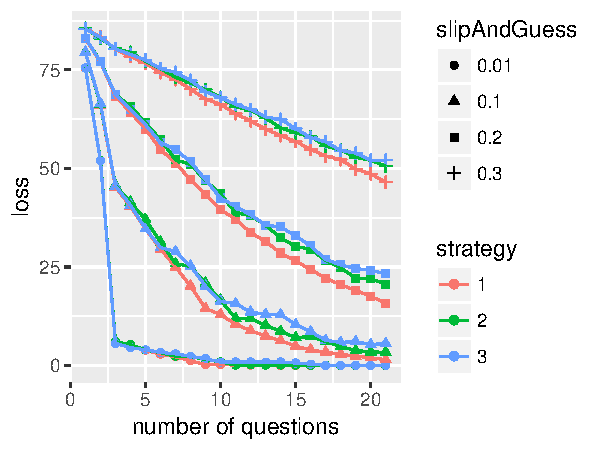
\includegraphics[width=\columnwidth]{simResults/LossStrategyComparisonThreeSkills.pdf}
  \end{center}
  \caption{Three Strategy Comparison on 3-skill case}  
  \label{fig:ComparisonThreeSkill}
\end{figure}

\begin{figure}[h!]
  \begin{center}
  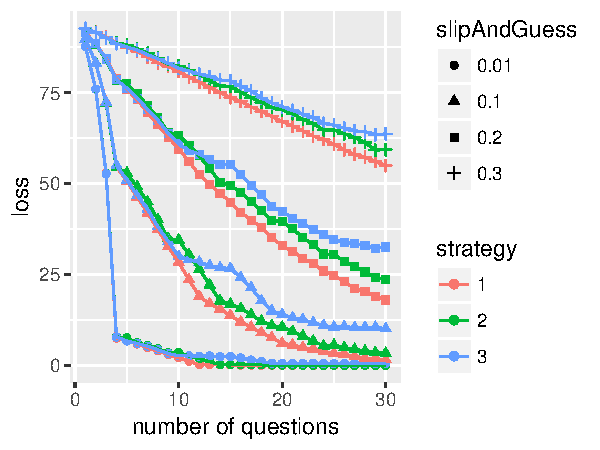
\includegraphics[width=\columnwidth]{simResults/LossStrategyComparisonFourSkills.pdf}
  \end{center}
  \caption{Three Strategy Comparison on 4-skill case}  
  \label{fig:ComparisonFourSkill}
\end{figure}

\begin{figure}[h!]
  \begin{center}
  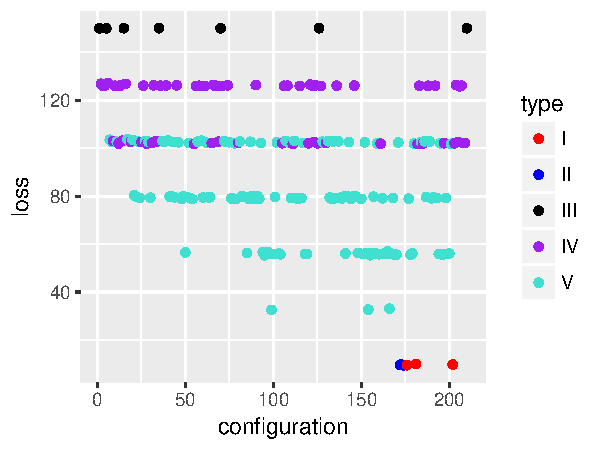
\includegraphics[width=\columnwidth]{simResults/LossBestConfig_theta001_J4.pdf}
  \end{center}
  \caption{3-skill case, slip=guess=0.01, J=4}  
  \label{fig:theta001J4ThreeSkill}
\end{figure}

\begin{figure}[h!]
  \begin{center}
  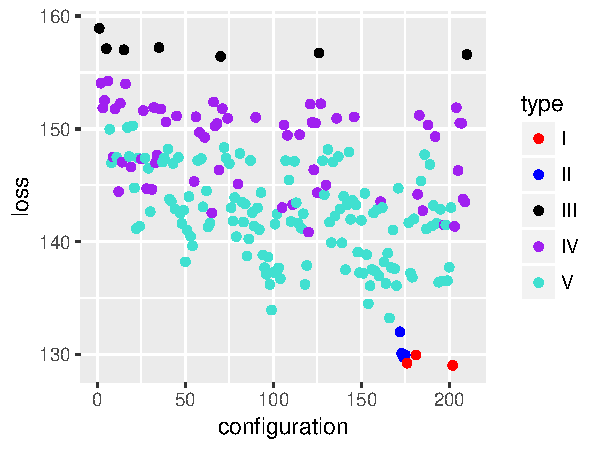
\includegraphics[width=\columnwidth]{simResults/LossBestConfig_theta02_J4.pdf}
  \end{center}
  \caption{3-skill case, slip=guess=0.2, J=4}  
  \label{fig:theta021J4ThreeSkill}
\end{figure}

\begin{figure}[h!]
  \begin{center}
  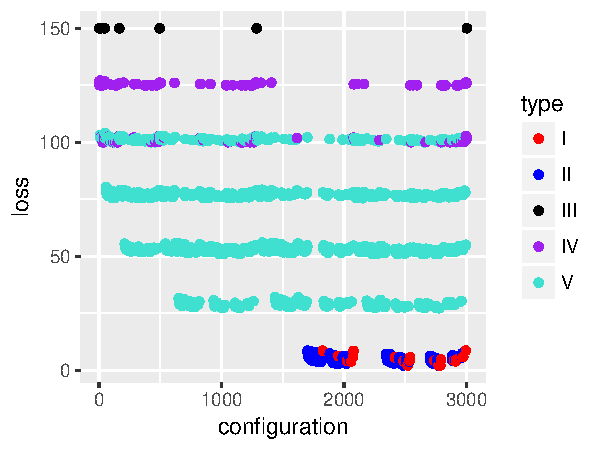
\includegraphics[width=\columnwidth]{simResults/LossBestConfig_theta001_J8.pdf}
  \end{center}
  \caption{3-skill case, slip=guess=0.01, J=8}  
  \label{fig:theta001J8ThreeSkill}
\end{figure}

\begin{figure}[h!]
  \begin{center}
  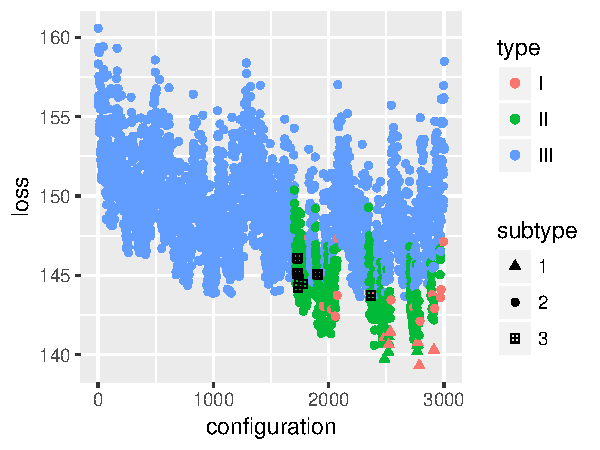
\includegraphics[width=\columnwidth]{simResults/LossBestConfig_theta03_J8.pdf}
  \end{center}
  \caption{3-skill case, slip=guess=0.3, J=8}  
  \label{fig:theta03J8ThreeSkill}
\end{figure}

\begin{figure}[h!]
  \begin{center}
  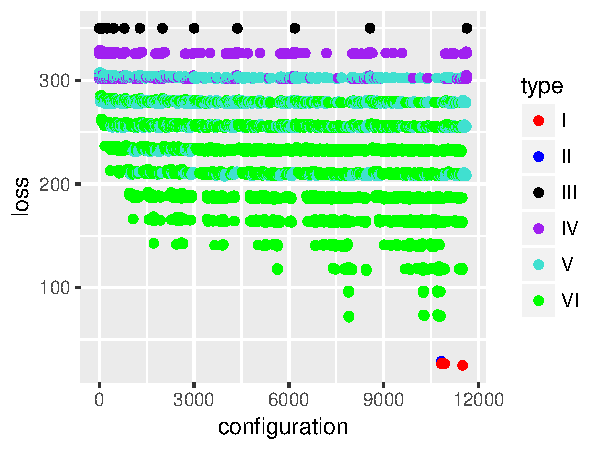
\includegraphics[width=\columnwidth]{simResults/Skill4LossBestConfig_theta001_J5.pdf}
  \end{center}
  \caption{4-skill case, slip=guess=0.01, J=5}  
  \label{fig:theta001J5FourSkill}
\end{figure}

\begin{figure}[h!]
  \begin{center}
  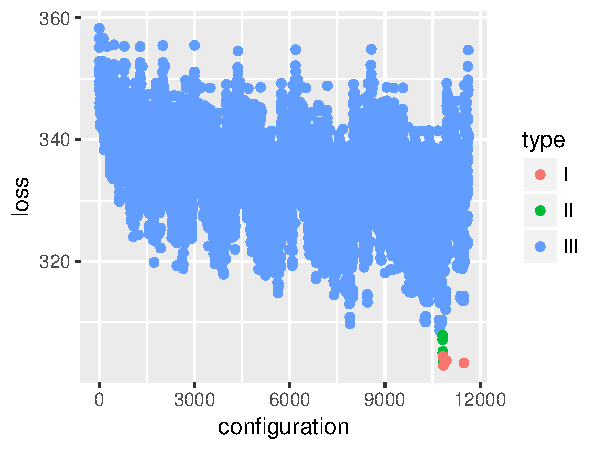
\includegraphics[width=\columnwidth]{simResults/Skill4LossBestConfig_theta02_J5.pdf}
  \end{center}
  \caption{4-skill case, slip=guess=0.2, J=5}  
  \label{fig:theta02J5FourSkill}
\end{figure}

%\begin{figure}[htbp]
%  \centering
%  \includesvg{theta02J5Total}
%  \caption{svg image}
%\end{figure}

\section{Discussion}
From the result in experiment 1 we can see that strategy 1 always works better than the other two strategies. 

From the result in experiment 2, when slip and guess parameters are as low as 0.01, we can see obvious graded patterns among different configurations. Those configuration that satisfies the identifiability requirement always work better than other configurations. There is no clear distinction between the configuration using only $e_{j}$ (the pure strategy) and those using at least one other q-vectors(mixed strategy). However, when slip and guess becomes higher, the pure strategy shows better than the mixed strategy.

Therefore, we argue that the best Q-matrix design is to use only the boolean unit vectors ${e_j}$ since it offers quicker convergence speed (as shown in experiment 1) and better robustness (as shown in experiment 2).

\section{Future Work}
More different experiments settings can be considered with different choice on student profiles distribution, and different number of skills involved. Besides, the case that slip and guess are unknown should also be considered, which involves a different identifiability requirement. Moreover, besides the empirical exploration, rigorous mathematical discussion can be done for the best Q-matrix design under DINA model. 
\bibliographystyle{apacite}
\bibliography{biblio}
\end{document}